Som tidligere diskuteret er processen for genetiske algoritmer følgende:

•	Forældre individerne bliver valgt.

•	Forældrene parres.

•	Populationen vokser.

•	Individerne bliver muteret, eller krydset.

•	Sandsynligheden for at en crossover eller mutation finder sted bliver bestemt ud fra en selektionsmetode.

I det følgende afsnit beskrives nogle af de selektionsmetoder der kan bruges. Det vil endvidere også blive diskuteret, hvilken af disse metoder der bedst kan anvendes til at producere skoleskemaer\cite{winston2014}.

\subsection{Roulette metoden}

Man kan forestille sig at hvert individ er tildelt et stykke på en roulette og størrelsen på stykket er proportional med individets fitness. Roulette bliver spinnet n antal gange, det vil tage for at vælge forældrene til den næste generation. Under hvert spin bliver individet under roulettens markør valgt til, at være en del af en gruppe af forældre til den næste generation. En kandidat kan godt blive valgt til, at være forældre flere gange, da det er forældrene til næste generation og ikke selve individerne i generationen, der bliver valgt, gør det dog ingen forskel. Formålet med denne metode er, at få valgt de forældre med den største fitness til næste generation, da de har større sandsynlig for, at skabe individer med større fitness. Problemet med denne metode er dog, at den genetiske algoritme hurtigt vil stå fast i den ene del af fitness rummet, da det er muligt at vælge den samme forældre flere gange, og derved kan der blive skabt en meget ensartet population, som gør at der kun vil blive udforsket et bestemt område af rummet i stedet for at udforske hele rummet\cite{jebari2013}\cite{selection}.
Roulette metoden kan illustreres på følgende måde:
\begin{figure}[!h]
  \centering
  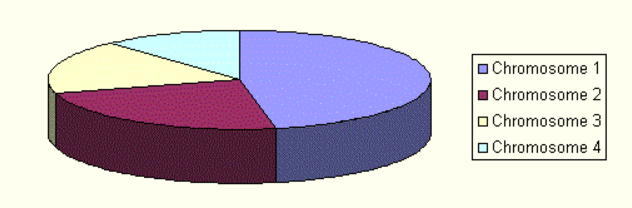
\includegraphics[width=\textwidth]{partials/graphics/roulette.png}
  \caption{Model over roulette metoden\cite{roulette}.}
  \label{fig:roulette}
\end{figure}

\subsection{Rank metoden}

I rang metoden bliver individerne sorteret efter størrelsen på deres fitness. Derefter bliver individerne tildelt lodder efter den plads de har fået efter sorteringen. Det vil sige at den med den laveste fitness får tildelt et lod, den med den anden mindste får tildelt to lodder osv. Antallet af lodder et individ er blevet tildelt forstørre chancen for at individet bliver valgt som forældre til en fremtidig generation. I modsætning til roulette metoden, har fitnessen altså i rang metoden en indirekte påvirkning på individernes chance for at bliver valgt.\cite{jebari2013} 

\subsection{Tournament metoden}

2 tilfældige individer bliver valgt fra populationen. Man generer en tilfældig værdi fra 0-1 for at sammenligne den med valgte sandsynlighedsværdi. Hvis værdien er mindre eller lige med sandsynlighedsværdien bliver det individ med højst fitness valgt ellers bliver individet med den lavere fitness valgt. Sandsynlighedsværdien bliver altid sat højere end 0.5 for at favorisere individet med den højeste fitness\cite{jebari2013}. 

I det følgende program benyttes roulette metoden. Ved brug af roulette metoden sikres det at der er større sandsynlighed for at individerne med den højeste fitness bliver brugt til at skabe de fremtidige generationer. 
